\subsection{Model}

\begin{figure}[h]
	\centering
	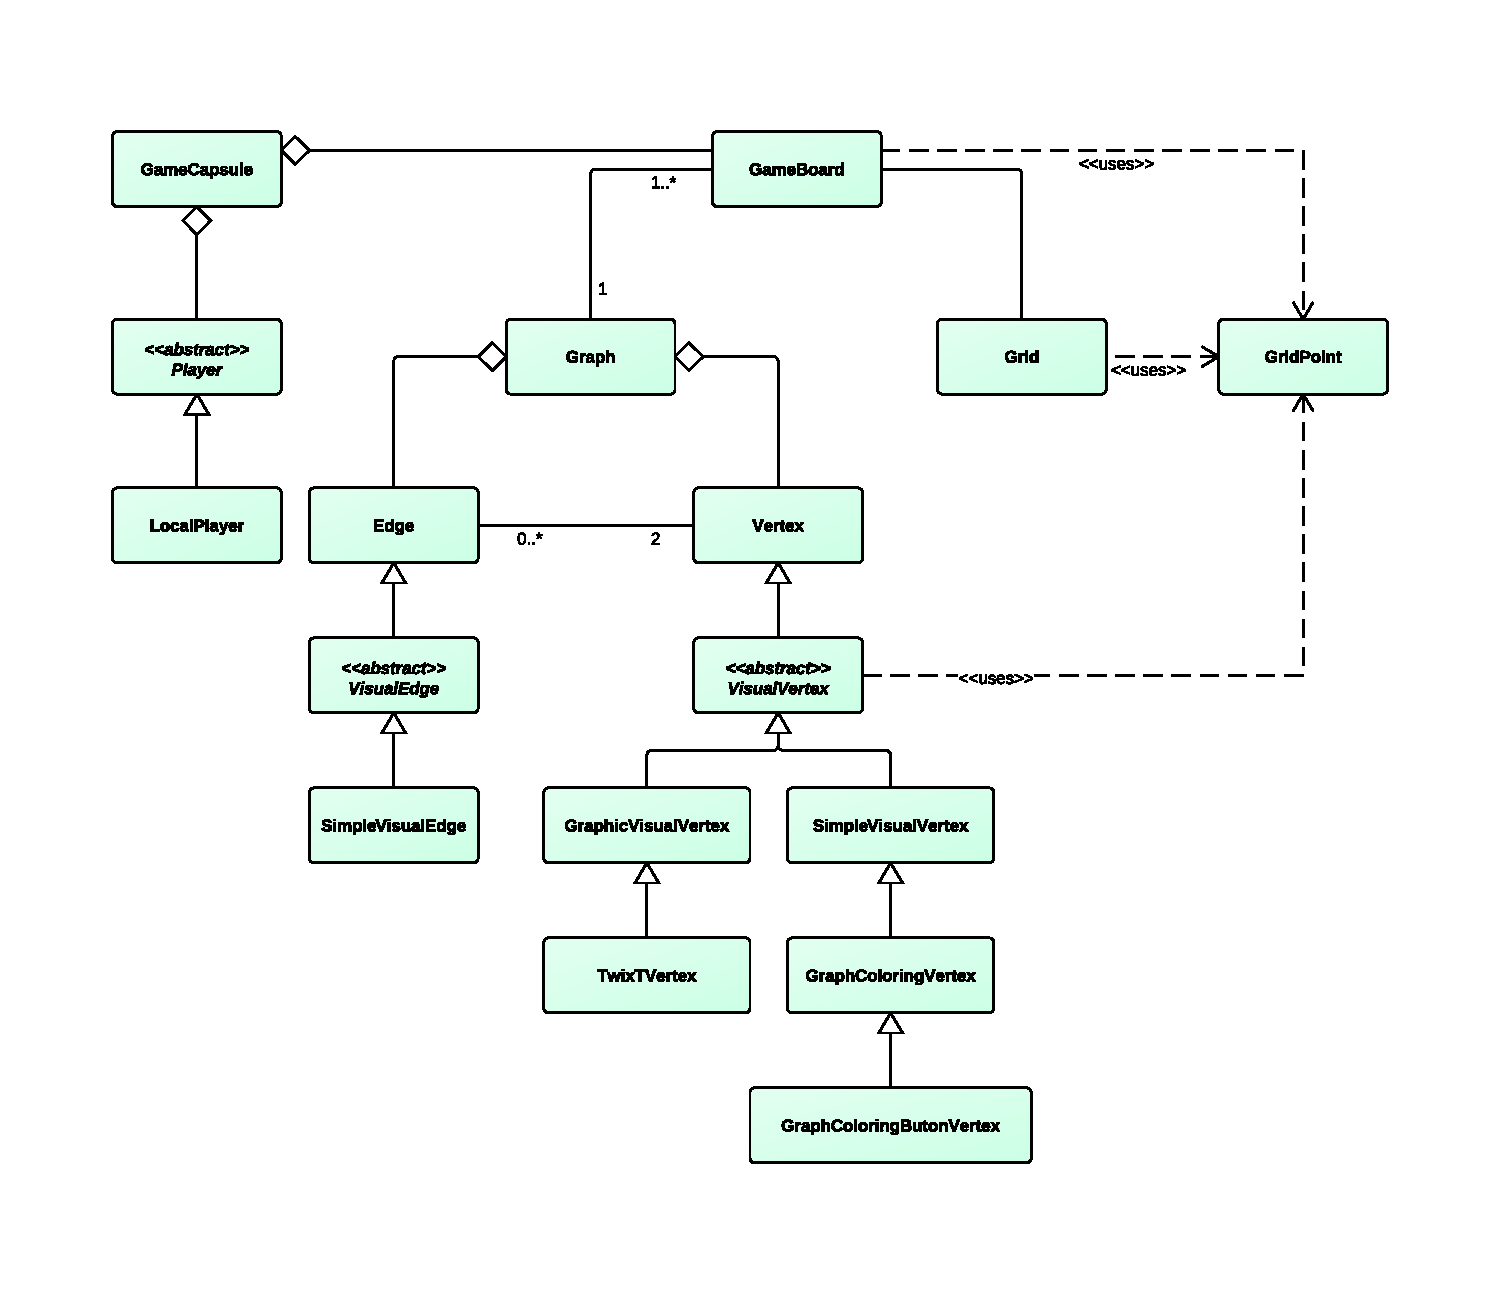
\includegraphics[page=1,width=\textwidth,keepaspectratio]{modelClassDiagram.pdf}
	\caption{Model class diagram.}
	\label{img:modelClassDiagram}
\end{figure}
\pagebreak

% GameBoard
\class{GameBoard}{gameboard}
This class represents the game board of a game. The \texttt{GameBoard} combines the logical \ref{cls:graph} with the \ref{cls:grid} and has access to both of them. \\

\centerdash

\paragraph*{Method Summary}
\paragraph*{}
\begin{longtable}{Lp{10cm}}
	\startmethodtable
	\method{public}{GameBoard(boolean isDirectedGraph)}{gb:gameboard} \\
	& Creates a new \texttt{GameBoard} with the specified option - if the \texttt{GameBoard} is directed or not. \\
	\method{public boolean}{addVisualVertex(VisualVertex visualVertex)}{gb:addvisualvertex} \\
	& Adds a \ref{cls:visualvertex} to this \texttt{GameBoard} and returns \texttt{true} if adding was successful. \\
	\method{public boolean}{addVisualVertices(Iterable<VisualVertex> visualVertices)}{gb:addvisualvertices} \\
	& Adds a list of \texttt{VisualVertices} to this \texttt{GameBoard} and returns \texttt{true} if adding was successful. \\
	\method{public VisualEdge}{addVisualEdge(VisualVertex vertexA, VisualVertex vertexB)}{gb:addvisualedge} \\
	& Adds a \ref{cls:visualedge} between two specified \texttt{VisualVertices} \texttt{vertexA} and \texttt{vertexB}, and returns the added \ref{cls:visualvertex}. \\
	\method{public boolean}{removeVisualVertex(VisualVertex visualVertex)}{gb:removevisualvertex} \\
	& Returns \texttt{true} if a specified \ref{cls:visualvertex} was removed successfully from this \texttt{GameBoard}. \\
	\method{public boolean}{removeVisualEdge(VisualEdge visualEdge)}{gb:removevisualedge} \\
	& Returns \texttt{true} if a specified \ref{cls:visualedge} was removed successfully from this \texttt{GameBoard}. \\
	\method{public VisualEdge}{getVisualEdge(VisualVertex vertexA, VisualVertex vertexB)}{gb:getVisualEdge} \\
	& Returns a \ref{cls:visualedge} between two specified \texttt{VisualVertices} \texttt{vertexA} and \texttt{vertexB}. \\
	\method{public boolean}{isDirectedGraph()}{gb:isdirectedgraph} \\
	& Returns \texttt{true} if the \ref{cls:graph} in this \texttt{GameBoard} is directed. \\
	\method{public Graph}{getGraph()}{gb:getgraph} \\
	& Returns the \ref{cls:graph} in this \texttt{GameBoard}. \\
	\method{public Grid}{getGrid()}{gb:getgrid} \\
	& Returns the \ref{cls:grid} in this \texttt{GameBoard}. \\
	\hline
\end{longtable}

\pagebreak

% Grid
\class{Grid}{grid}
This class represents the \gls{grid}, on which the \ref{cls:graph} will be located. \\

\centerdash

\paragraph*{Method Summary}
\paragraph*{}
\begin{longtable}{Lp{10cm}}
	\startmethodtable
	\method{public}{Grid(int horizontalGridPoints, int verticalGridPoints)}{grid:grid} \\
	& Creates a new \texttt{Grid} with the specified parameters. \\
	\method{public boolean}{addVisualVertexToGrid(VisualVertex visualVertex)}{grid:addvisualvertextogridpoint} \\
	& Returns \texttt{true} if a specified \ref{cls:visualvertex} was added successfully to this \texttt{Grid}. \\
	\method{public boolean}{removeVisualVertexAtGridPoint(GridPoint gridPoint)}{grid:removevisualvertexatgridpoint} \\
	& Returns \texttt{true} if a \ref{cls:visualvertex} was removed successfully from the specified \ref{cls:gridpoint} on this \texttt{Grid}. \\
	\method{public VisualVertex}{getVisualVertexAtGridPoint(GridPoint gridPoint)}{grid:getvisualvertexatgridpoint} \\
	& Returns a \ref{cls:visualvertex} from the specified \ref{cls:gridpoint} on this \texttt{Grid}. \\
	\hline
\end{longtable}

\pagebreak

% GridPoint
\class{GridPoint}{gridpoint}
This class represents a grid point on the \ref{cls:grid}, which basically is a coordinate, on which \texttt{vertices} will be located. \\

\centerdash

\paragraph*{Method Summary}
\paragraph*{}
\begin{longtable}{Lp{10cm}}
	\startmethodtable
	\method{public}{GridPoint(int positionX, int positionY)}{gp:gridpoint} \\
	& Creates a new \texttt{GridPoint} with the specified positions \texttt{positionX} and \texttt{positionY}. \\
	\method{public int}{getPositionX()}{gp:getpositionx} \\
	& Returns the x coordinate of the \texttt{GridPoint}. \\
	\method{public int}{getPositionY()}{gp:getpositiony} \\
	& Returns the y coordinate of the \texttt{GridPoint}. \\
	\hline
\end{longtable}

\pagebreak

% Graph
\class{Graph}{graph}
This class represents the logical \gls{graph}. \\

\centerdash

\paragraph*{Method Summary}
\paragraph*{}
\begin{longtable}{Lp{10cm}}
	\startmethodtable
	\method{public boolean}{addEdge(Vertex vertexA, Vertex vertexB)}{graph:addEdge} \\
	& Adds an \ref{cls:edge} to this \texttt{Graph}. \\
	\method{public boolean}{addVertex(Vertex vertex)}{graph:addVertex} \\
	& Adds a \ref{cls:vertex} to this \texttt{Graph}. \\
	\method{public boolean}{removeVertex(Vertex vertex)}{graph:removevertex} \\
	& Removes a specified \ref{cls:vertex} from this \texttt{Graph} and the \ref{cls:edge}s connected to it. \\
	\method{public boolean}{removeEdge(Edge edge)}{graph:removeedge} \\
	& Removes a specified \ref{cls:edge} from this \texttt{Graph}. \\
	\method{public Iterable<Vertex>}{getVertices()}{graph:getvertices} \\
	& Returns an iterable list of the \texttt{Vertices} of this \texttt{Graph}.  \\
	\method{public Iterable<Edge>}{getEdges()}{graph:getedges} \\
	& Returns an iterable list of the \ref{cls:edge}s of this \texttt{Graph}. \\
	\hline
\end{longtable}

\pagebreak

% Vertex
\class{Vertex}{vertex}
This class represents a logical \gls{vertex}. \\

\subclasses{cls:visualvertex}

\centerdash

\paragraph*{Method Summary}
\paragraph*{}
\begin{longtable}{Lp{10cm}}
	\startmethodtable
	\method{public Iterable<Vertex>}{getAdjacentVertices()}{vertex:getadjacentvertices} \\
	& Returns all \texttt{Vertices} that are connected to this \texttt{Vertex}. \\
	\method{public UUID}{getUID()}{vertex:getuid} \\
	& Returns the unique identifier for this \texttt{Vertex}. \\
	\method{public Iterable<Edge>}{getIncomingEdges()}{vertex:getincomingedges} \\
	& Returns an iterable list of incoming \ref{cls:edge}s. \\
	\method{public boolean}{addIncomingEdge(Edge edge)}{vertex:addincomingedge} \\
	& Adds an incoming \ref{cls:edge} to the list of incoming \ref{cls:edge}s. \\
	\method{public boolean}{removeIncomingEdge(Edge edge)}{vertex:removeincomingedge} \\
	& Removes an incoming \ref{cls:edge} from the list of incoming \ref{cls:edge}s. \\
	\method{public Iterable<Edge>}{getOutgoingEdges()}{vertex:getoutgoingedges} \\
	& Returns an iterable list of outgoing \ref{cls:edge}s. \\	
	\method{public boolean}{addOutgoingEdge(Edge edge)}{vertex:addoutgoingedge} \\
	& Adds an outgoing \ref{cls:edge} to the list of outgoing \ref{cls:edge}s. \\
	\method{public boolean}{removeOutgoinggEdge(Edge edge)}{vertex:removeoutgoingedge} \\
	& Removes an outgoing \ref{cls:edge} from the list of outgoing \ref{cls:edge}s. \\
	\method{public boolean}{isAdjacentTo(Vertex vertex)}{vertex:isadjacentto} \\
	& Returns true if this \texttt{Vertex} is adjacent to the given \texttt{Vertex}. \\
	\hline
\end{longtable}

\pagebreak

% VisualVertex
\abstractclass{VisualVertex}{visualvertex}
\createindentedlist{de.graphioli.model.Vertex, de.graphioli.model.VisualVertex}

This class represents a \gls{vertex} with its graphical representation. \\

\subclasses{cls:graphicvisualvertex, cls:simplevisualvertex}

\centerdash

\paragraph*{Method Summary}
\paragraph*{}
\begin{longtable}{Lp{10cm}}
	\startmethodtable
	\method{public}{VisualVertex(GridPoint gridPoint)}{vv:visualvertex} \\
	& Creates a new \texttt{VisualVertex} and places it on the specified \ref{cls:gridpoint}. \\
	\method{protected abstract boolean}{draw(Graphics2D)}{vv:draw} \\
	& Draws the \texttt{VisualVertex} onto the given \texttt{Graphics2D} object. \\
	\method{final void}{update()}{vv:update} \\
	& Updates the graphical representation of this \texttt{VisualVertex} by recreating its \texttt{BufferedImage} using the \ref{vv:draw} method.\\ 
	\method{public GridPoint}{getGridPoint()}{vv:getgridpoint} \\
	& Returns the \ref{cls:gridpoint} of this \texttt{VisualVertex}. \\ 
	\method{public boolean}{setGridPoint(GridPoint gridPoint)}{vv:setgridpoint} \\
	& Sets the \ref{cls:gridpoint} of this \texttt{VisualVertex}. \\
	\method{public final BufferedImage}{getBufferedImage()}{vv:getbufferedimage} \\
	& Returns the \texttt{BufferedImage}, which contains the current graphical representation of this \texttt{VisualVertex}. \\ 
	\hline
\end{longtable}

\pagebreak

% SimpleVisualVertex
\class{SimpleVisualVertex}{simplevisualvertex}
\createindentedlist{de.graphioli.model.Vertex, de.graphioli.model.VisualVertex, de.graphioli.model.SimpleVisualVertex}

This class represents a simple \ref{cls:visualvertex} with predefined attributes.\\

\subclasses{cls:graphcoloringvertex}

\centerdash

\paragraph*{Method Summary}
\paragraph*{}
\begin{longtable}{Lp{10cm}}
	\startmethodtable
	\method{public Color}{getColor()}{svv:getcolor} \\
	& Returns the \texttt{color} of this \texttt{SimpleVisualVertex}. \\
	\method{public int}{getStrokeWeight()}{svv:getStrokeWeight} \\
	& Returns the \texttt{stroke weight} of this \texttt{SimpleVisualVertex}. \\
	\method{public Color}{getStrokeColor()}{svv:getstrokecolor} \\
	& Returns the \texttt{stroke color} of this \texttt{SimpleVisualVertex}. \\
	\method{public boolean}{setColor(Color color)}{svv:setcolor} \\
	& Sets the \texttt{color} of this \texttt{SimpleVisualVertex}. \\
	\method{public boolean}{setStrokeWeight(int strokeWeight)}{svv:setstrokeweight} \\
	& Sets the \texttt{stroke weight} of this \texttt{SimpleVisualVertex}. \\
	\method{public boolean}{setStrokeColor(Color strokeColor)}{svv:setstrokecolor} \\
	& Sets the \texttt{stroke color} of this \texttt{SimpleVisualVertex}. \\
	\method{protected void}{draw(Graphics2D)}{svv:draw} \\
	& Draws this \texttt{SimpleVisualVertex} according to its \texttt{color}, \texttt{stroke color} and \texttt{stroke weight} attributes. \\
	\hline
\end{longtable}

\pagebreak

% GraphColoringVertex
\class{GraphColoringVertex}{graphcoloringvertex}
\createindentedlist{de.graphioli.model.Vertex, de.graphioli.model.VisualVertex, de.graphioli.model.SimpleVisualVertex, de.graphioli.model.GraphColoringVertex}

This class represents a \gls{vertex} used in the \graphcoloring \gls{game} by defining a \texttt{colorID} attribute that can be used by the \graphcoloring \gls{algorithm}s. \\

\subclasses{cls:graphcoloringbuttonvertex}	

\centerdash

\paragraph*{Method Summary}
\paragraph*{}
\begin{longtable}{Lp{10cm}}
	\startmethodtable
	\method{public int}{getColorID()}{gcv:getcolorid} \\
	& Returns the \texttt{color identification} of this \texttt{GraphColoringVertex}. \\
	\method{public boolean}{setColorID(int id)}{gcv:setcolorid} \\
	& Sets the \texttt{color identification} of this \texttt{GraphColoringVertex} and changes its \texttt{Color} attribute accordingly. \\
	
	\hline
\end{longtable}

\pagebreak

% GraphColoringButtonVertex
\class{GraphColoringButtonVertex}{graphcoloringbuttonvertex}
\createindentedlist{de.graphioli.model.Vertex, de.graphioli.model.VisualVertex, de.graphioli.model.SimpleVisualVertex, de.graphioli.model.GraphColoringVertex, de.graphioli.model.GraphColoringButtonVertex}

This class represents a special \ref{cls:graphcoloringvertex} that serves as a button for selecting a color. \\ 

\centerdash

\paragraph*{Method Summary}
\paragraph*{}
\begin{longtable}{Lp{10cm}}
	\startmethodtable
	\method{public boolean}{isHighlighted()}{gcbv:ishighlighted} \\
	& Returns \texttt{true} if this \texttt{GraphColoringButtonVertex} is selected. \\
	\method{public boolean}{setHighlighted(boolean isHighlighted)}{gcbv:sethighlighted} \\
	& Sets the \texttt{highlighted} attribute of this \texttt{GraphColoringVertex} and changes its \texttt{stroke color} to visually represent the current state. \\
	\hline
\end{longtable}

\pagebreak

% GraphicVisualVertex
\class{GraphicVisualVertex}{graphicvisualvertex}
\createindentedlist{de.graphioli.model.Vertex, de.graphioli.model.VisualVertex, de.graphioli.model.GraphicVisualVertex}
This class represents a \ref{cls:visualvertex} with a custom icon. \\

\subclasses{cls:twixtvertex}

\centerdash

\paragraph*{Method Summary}
\paragraph*{}
\begin{longtable}{Lp{10cm}}
	\startmethodtable
	\method{public}{GraphicVisualVertex(String fileName)}{gvv:graphicvisualvertexfile} \\
	& Creates a new \texttt{GraphicVisualVertex} using the image in the specified file as icon. \\
	\method{public}{GraphicVisualVertex(BufferedImage image)}{gvv:graphicvisualverteximage} \\
	& Creates a new \texttt{GraphicVisualVertex} using the specified \texttt{BufferedImage} as icon. \\
	\method{public BufferedImage}{getImage()}{gvv:getimage} \\
	& Returns the \texttt{image} that represents this \texttt{GraphicVisualVertex}. \\
	\method{public boolean}{setImage(BufferedImage image)}{gvv:setimage} \\
	& Sets the \texttt{image} that represents this \texttt{GraphicVisualVertex}. \\
	\method{protected final BufferedImage}{loadBufferedImage(String fileName)}{gvv:loadbufferedimage} \\
	& Loads the image file at the given \texttt{fileName} and returns it as a \texttt{BufferedImage}. \\
	\method{protected void}{draw(Graphics2D)}{svv:draw} \\
	& Draws this \texttt{GraphicVisualVertex} using its specified \texttt{image}. \\
	\hline
\end{longtable}

\pagebreak

% TwixtVertex
\class{TwixTVertex}{twixtvertex}
\createindentedlist{de.graphioli.model.Vertex, de.graphioli.model.VisualVertex, de.graphioli.model.GraphicVisualVertex,  de.graphioli.model.TwixtVertex}
This class represents a \gls{vertex} used in the \twixt game, which is displayed as either a red or blue tower, depending on the \gls{player} it belongs to. \\

\centerdash

\paragraph*{Method Summary}
\paragraph*{}
\begin{longtable}{Lp{10cm}}
	\startmethodtable
	\method{public}{TwixtVertex(int playerID)}{tv:twixtvertex} \\
	& Creates a new \texttt{TwixtVertex} and associates it with the \ref{cls:player} of the given \texttt{playerID}. \\
	\method{public int}{getPlayerID()}{tv:getplayerid} \\
	& Returns the \ref{cls:player}'s identification. \\
	\method{public static boolean}{init(int redPlayerID, int bluePlayerID)}{tv:init} \\
	& Initializes the \texttt{TwixtVertex} by loading the images and defining which ID belongs to the red and blue \ref{cls:player} respectively. \\
	\hline
\end{longtable}

\pagebreak

% Edge
\class{Edge}{edge}
This class represents a logical \gls{edge}. \\

\subclasses{cls:visualedge}

\centerdash

\paragraph*{Method Summary}
\paragraph*{}
\begin{longtable}{Lp{10cm}}
	\startmethodtable
	\method{public}{Edge(Vertex vertexA, Vertex vertexB)}{edge:edge} \\
	& Creates a new \texttt{Edge} with the specified \texttt{Vertices} \texttt{vertexA} and \texttt{vertexB}. \\
	\method{public Vertex}{getOriginVertex()}{edge:getoriginvertex} \\
	& Returns the origin \ref{cls:vertex}. \\
	\method{public Vertex}{getTargetVertex()}{edge:gettargetvertex} \\
	& Returns the target \ref{cls:vertex}. \\
	\method{public int}{getWeight()}{edge:getweight} \\
	& Returns the \texttt{weight} of this \texttt{Edge}. \\
	\method{public boolean}{setWeight(int weight)}{edge:setweight} \\
	& Sets the \texttt{weight} of this \texttt{Edge}. \\
	\hline
\end{longtable}

\pagebreak

% VisualEdge
\abstractclass{VisualEdge}{visualedge}
\createindentedlist{de.graphioli.model.Edge, de.graphioli.model.VisualEdge}
This class represents an \gls{edge} with its visual representation.

\subclasses{cls:simplevisualedge}

\centerdash

\paragraph*{Method Summary}
\paragraph*{}
\begin{longtable}{Lp{10cm}}
	\startmethodtable
	\method{protected abstract boolean}{draw(Graphics2D)}{ve:draw} \\
	& Draws the \texttt{VisualEdge} onto the given \texttt{Graphics2D} object. \\
	\method{final void}{update()}{ve:update} \\
	& Updates the graphical representation of this \texttt{VisualEdge} by recreating its \texttt{BufferedImage} using the \ref{ve:draw} method.\\ 
	\method{public final BufferedImage}{getBufferedImage()}{ve:getbufferedimage} \\
	& Returns the \texttt{BufferedImage}, which contains the current graphical representation of this \texttt{VisualEdge}. \\ 
	\hline
\end{longtable}



\pagebreak

% SimpleVisualEdge
\class{SimpleVisualEdge}{simplevisualedge}
\createindentedlist{de.graphioli.model.Edge, de.graphioli.model.VisualEdge, de.graphioli.model.SimpleVisualEdge}

This class represents a simple \ref{cls:visualedge} with predefined attributes. \\

\centerdash

\paragraph*{Method Summary}
\paragraph*{}
\begin{longtable}{Lp{10cm}}
	\startmethodtable
	\method{public Color}{getColor()}{sve:getcolor} \\
	& Returns the \texttt{color} of this \texttt{SimpleVisualEdge}. \\
	\method{public int}{getStrokeWeight()}{sve:getstrokeweight} \\
	& Returns the \texttt{stroke weight} of this \texttt{SimpleVisualEdge}. \\
	\method{public boolean}{setColor(Color color)}{sve:setcolor} \\
	& Sets the \texttt{color} of this \texttt{SimpleVisualEdge}. \\
	\method{public int}{setStrokeWeight()}{sve:setstrokeweight} \\
	& Sets the \texttt{stroke weight} of this \texttt{SimpleVisualEdge}. \\
	\method{protected void}{draw(Graphics2D)}{sve:draw} \\
	& Draws this \texttt{SimpleVisualEdge} according to its stroke color and stroke weight attributes and the position of its \texttt{VisualVertices}. \\
	\hline
\end{longtable}

\pagebreak

% Player
\abstractclass{Player}{player}
This class represents a \gls{player}. \\

\subclasses{cls:localplayer}

\centerdash

\paragraph*{Method Summary}
\paragraph*{}
\begin{longtable}{Lp{10cm}}
	\startmethodtable
	\method{public}{Player(String name)}{player:player} \\
	& Creates a new \texttt{Player} with the specified \texttt{name}. \\
	\method{public UUID}{getUID()}{player:getuid} \\
	& Returns the \texttt{UUID} of this \texttt{Player}. \\
	\method{public String}{getName()}{player:getname} \\
	& Returns the \texttt{name} of this \texttt{Player}. \\
	\hline
\end{longtable}

% LocalPlayer
\class{LocalPlayer}{localplayer}
\createindentedlist{de.graphioli.model.Player, de.graphioli.model.LocalPlayer}
This class represents a local \gls{player}.

\pagebreak

% GameCapsule
\class{GameCapsule}{gamecapsule}
This serializable class represents a \texttt{GameCapsule} that holds all the important data about the game state. A \gls{savegame} will be saved in such a \texttt{GameCapsule}, which later on can be loaded to resume the \gls{game}.

\centerdash

\paragraph*{Method Summary}
\paragraph*{}
\begin{longtable}{Lp{10cm}}
	\startmethodtable
	\method{public}{GameCapsule(GameBoard board, Iterable<Player> player, Player activePlayer)}{gc:gamecapsule} \\
	& Creates a new \texttt{GameCapsule} with the specified parameters. \\
	\method{public GameBoard}{getBoard()}{gc:getboard} \\
	& Returns the \ref{cls:gameboard} of this \texttt{GameCapsule}. \\
	\method{public Iterable<Player>}{getPlayers()}{gc:getplayers} \\
	& Returns an iterable list of \ref{cls:player}s of this \texttt{GameCapsule}. \\
	\method{public Player}{getActivePlayer()}{gc:getactiveplayer} \\
	& Returns the current active \ref{cls:player} of this \texttt{GameCapsule}. \\
	\hline
\end{longtable}